\section{Learning Refinement Distributions}
Randomized refinement provides us with a framework to learn a policy that implements
\textsc{NDGetInstantiation} and performs well empirically. Our approach applies RL
to train continuous proposal distributions for symbolic reference instantiations, in order
to implement this routine.

\subsection{Formulation as Reinforcement Learning Problem}
We formulate plan refinement as an MDP as follows:
\begin{tightlist}
\item A state $s \in \St$ is a tuple $(\pi, \sigma, E, n)$, consisting of the
high-level plan, its current setting of values for symbolic references,
the geometric environment encoding, and a counter for
the number of calls to the sampler.
\item An action $a \in \A$ is a pair $(p, x)$, where $p$ is the discrete symbolic
reference to resample and $x$ is the continuous value assigned to $p$ in the new refinement.
\item The transition function $T(s, a, s')$ is split up into 3 cases. In all cases, $n$ increases by 1. $L$ refers to
the number of samples for one planning problem, encompassing both the task planning problem
and the environment.
  \begin{tightlist}
  \item Case 1: $n > L$. We sample a new state from $\Prob$ and reset $n$ to 0.
  \item Case 2: the proposed value $x$ is IK infeasible. The state remains the same.
  \item Case 3: Otherwise, the value of $p$ is set to $x$ and the motion planner is called.
  \end{tightlist}
\item The reward function $R(s, a, s')$ provides rewards based on a measure of closeness to a valid plan refinement.
\item $\Prob$ is a distribution over planning problems, thus defining the initial state distribution for this MDP.
\end{tightlist}

We restrict our attention to training policies that suggest $x$ for actions in $\A$.
We note that randomized refinement already provides a fixed policy for selecting $p$.

Our reward function $R$ explicitly encourages successful plan refinement, providing positive reward linearly
interpolated between 0 and 20 based on the fraction of high-level actions whose preconditions are
satisfied. Additionally, we give $-1$ reward every time we sample an IK infeasible pose.

\begin{figure}[t]
  \centering
    \noindent
    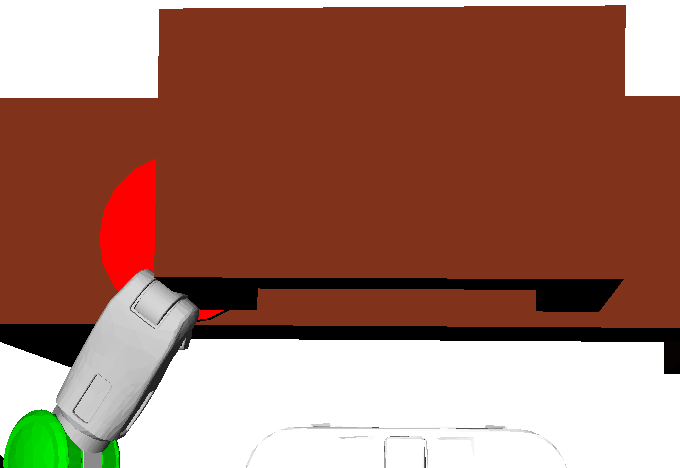
\includegraphics[scale=0.15]{images/fry_bad_grasp_pd1.png}\hspace{6mm}
    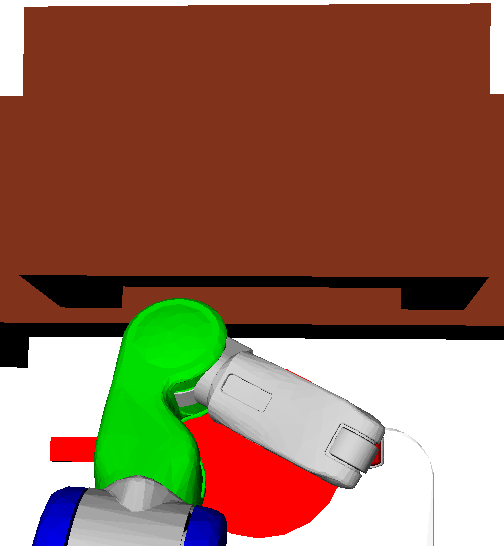
\includegraphics[scale=0.15]{images/fry_bad_grasp_pd2.png}
    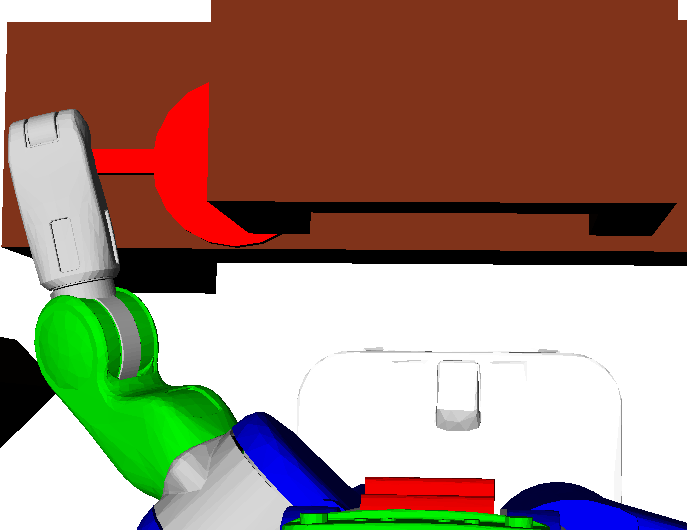
\includegraphics[scale=0.16]{images/fry_good_grasp_bad_pd.png}\hspace{6mm}
    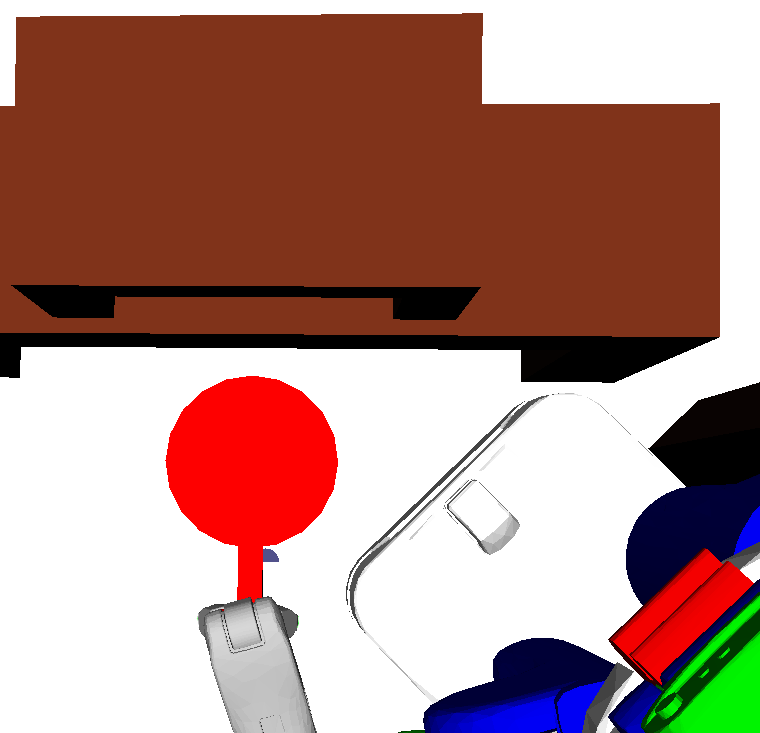
\includegraphics[scale=0.13]{images/fry_good_grasp_good_pd.png}
  \caption{\small{\textbf{Top}: When the frying pan is not grasped by the handle, any attempted putdown pose for
placing it into the narrow shelf fails. \textbf{Bottom}: When the frying pan is grasped by the handle, some putdown
poses may succeed, as in the right, and some may fail, as in the left. In general, delayed rewards
are important in the plan refinement MDP; sometimes multiple symbolic references require resampling to
change an infeasible refinement into a feasible one.}}
  \label{fig:delayed}
\end{figure}

\subsection{Training Process}
We learn a policy for this MDP by adapting the method of Zucker et al.~\cite{workspacebias}, which
uses a linear combination of features to define a distribution over poses. In our setting, we learn a weight
vector $\theta_{p}$ for each reference \emph{type}, comprised of a pose type and possibly a gripper
(e.g., ``left gripper grasp pose,'' ``right gripper putdown pose,'' ``base pose'').
This decouples the learned distributions from any single high-level plan and allows generalization across problem instances.

We develop a feature function $f(s, a) = f(s, p, x)$ that maps the current
state $s \in \St$ and action $a \in \A$ to a
feature vector; $f$ defines a policy class for the MDP. Additionally, we define
$N$ as the number of planning problems on which to train and
$\epsilon$ as the number of samples comprising a training episode, after which we update weights.

The training is a natural extension of randomized
refinement and progresses as follows. $N$ times, sample from $\Prob$ to obtain
a complete planning problem $\Pi$. For each $\Pi$, run the randomized refinement
algorithm to attempt to find a valid plan refinement, allowing the \textsc{Resample}
routine to be called $L$ times before termination. Select actions according to the $\theta_{p}$
and collect rewards according to $R$. After every $\epsilon$ calls to
\textsc{Resample}, perform a gradient update on the weights.

Our weight vectors are initialized to $\vec{\mathbf{0}}$ for all plan parameter types -- this
initialization represents a uniform distribution across the limits of the geometric search space.
We use 24 features for learning the $\theta_{p}$. 9 binary features encode the bucketed distance between the sample
and target (the object referenced by the parameter). 9 binary features encode the bucketed sample height. 3 features
describe the number of other objects within discs of radius 7, 10, and 15 centimeters around the
sample. 3 binary features describe the angle made between the vector from the
robot to the target and the vector from the sample to the target: whether the angle is less than
$\pi/3$, $\pi/2$, and $3\pi/4$.

\figref{fig:delayed} shows that delayed rewards are an important
aspect of the MDP: if a grasping pose along the lip of the frying pan is sampled, no putdown pose can lead
to it being placed inside the shelf. Typically, an infeasible refinement must undergo
resampling for several distinct symbolic references in order to reach a feasible refinement.

\subsection{Distribution and Gradient Updates}
We adopt the sampling distribution used in Zucker et al.~\cite{workspacebias}
for a symbolic reference $p$ with sample value $x$, in state $s \in \St$:
$$q(s, p, x) \propto \exp(\theta_{p}^{T} f(s, p, x)).$$
We define the expected reward of an episode $\xi$:
$$\eta(\theta_{p}) = \mathbb{E}_{q}[R(\xi)]$$ and approximate its gradient:
$$\nabla \eta(\theta_{p}) \approx \frac{R(\xi)}{\epsilon} \sum_{i=1}^{\epsilon}(f(s, p, x_{i}) - \mathbb{E}_{q,s}[f]).$$
$R(\xi)$ is the sum over all rewards obtained throughout $\xi$, and
$\mathbb{E}_{q,s}[f]$ is the expected feature vector under $q$ in state $s$. The weight vector update is then:
$$\theta_{p} \leftarrow \theta_{p} + \alpha \nabla \eta(\theta_{p})$$
for appropriate step size $\alpha$.

We sample $x$ from $q$ using the Metropolis algorithm~\cite{chib1995understanding}.
Since our distributions are continuous, we cannot easily calculate $\mathbb{E}_{q}[f]$,
so we approximate it by averaging together the feature vectors for several samples from $q$.